\lecture{10}{March 3 01:10}{}
\chapter{Finite Barriers}
\section{Finite Square Well}

\begin{figure}[H]
	\centering
	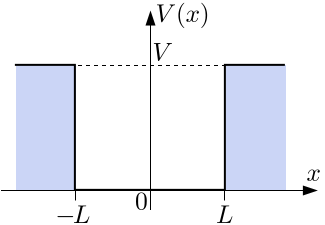
\includegraphics[width=0.4\textwidth]{Figures/03.png}
	\caption{}
	\label{fig:}
\end{figure}

We look here at cases where 
\[
	E > V_0
\]
\begin{figure}[H]
	\centering
	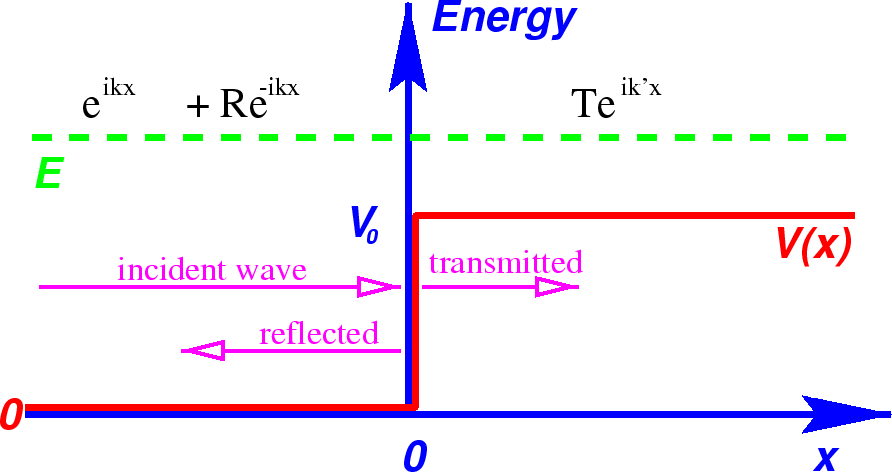
\includegraphics[width=0.5\textwidth]{Figures/04.png}
	\caption{}
	\label{fig:}
\end{figure}
For the solution in between we have that we get to solutions of \(\frac{1}{k_0}\) and \(\frac{1}{k^{\prime} }\). And 
in order to find a solution we have to match the boundary conditions at \(\frac{a}{2}\). Thus, what we are doing is solving for a real 
\(k_0\) with a moving wave packet.  Suppose we had Region 1 and 2 where 
\[
	\psi _1(x) = A e^{ik_1 x} + Be^{-ik_1 x}  
\]
which represents the incoming and outcoming wave where \(k= \sqrt{\frac{2mE}{\hbar ^{2} }} \). We will now make the assumption that in region 2 we ignore the wave coming back where
\[
	\psi _2 (x) = Ce^{ik_2 x} 
\] 
Thus, we are asking the equation of how much of the wave is going to be coming through. The \(B\) coefficient is a reflection and the 
\(C\) coefficient is the transmission. We are assuming that there is no particle coming in, thus we ignore the \(D\) term. Therefore
\[
	k_2 = \sqrt{2m\frac{E-V_0}{\hbar ^{2} }} 
\]
To solve, shift the solution to the left. Our first boundary condition is 
\[
	\psi _1(x=0) = \psi _2 (x=0) \implies A + B = C
\]
\[
	\frac{\mathrm{d}\psi_1}{\mathrm{d}x} (x=0) = \frac{\mathrm{d}\psi _2}{\mathrm{d}x} (x=0)  \implies ik_1(A-B) = ik_2 C
\]
\begin{remark}
	Notice 2 equations and 3 unknowns. However, depending on the wavepacket for a given \(k\) we know what \(A\) is.  
	Thus we are going to be computing ratios between \(A,B,C\) 
\end{remark}

\[
	A- B = \frac{k_2}{k_1} C
\]
Solving we must have
\[
	2A = C  \left( 1+\frac{k_2}{k_1} \right) 
\]
\[
	\frac{C}{A} = \frac{2k_1}{k_{1} + k_2 }
\]
\[
	\frac{B}{A}= \frac{k_{1}-k_2 }{k_1 + k_2}
\]
Let \(\mathcal{R} = \vert \frac{B}{A} \vert ^{2} \) 
\[
	\gamma = \frac{k_2}{k_1} \implies  \mathcal{R}  = \frac{(1- \gamma)^{2} }{(1 + \gamma)^{2} }
\]
To get the probability of transmission is simply
\[
	\mathcal{T} = 1 - \mathcal{R} = \frac{4\gamma}{(1+\gamma)^{2} }
\]
Notice that \(\gamma = \sqrt{\frac{E-V_0}{E}}  \). When this quantity \( \neq  0 \)  , then there is a finite reflection. Classically speaking, 
if a particle passes through there should be no reflection i.e. a particle rolling with enough energy. In the quantum case, this is not true. We can now graph these quantities to show 

\begin{figure}[H]
	\centering
	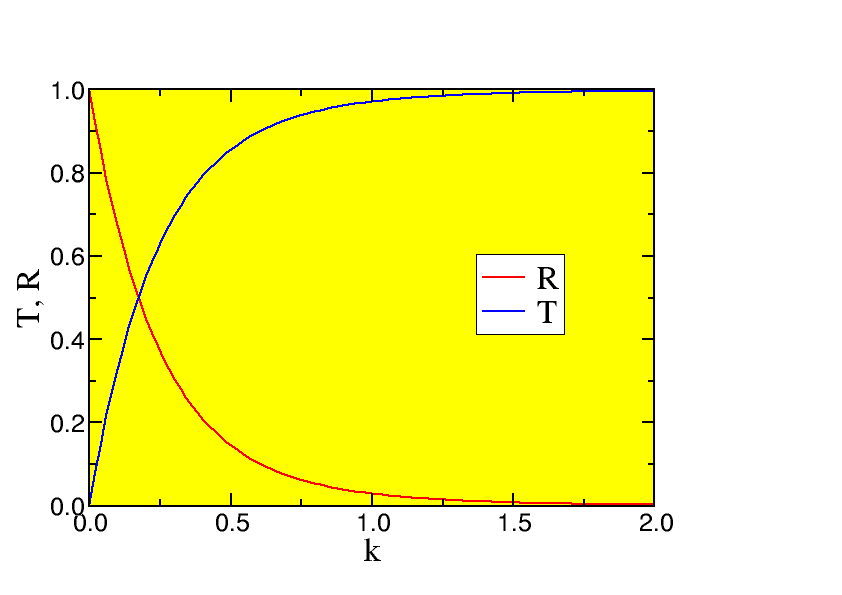
\includegraphics[width=0.5\textwidth]{Figures/05.png}
	\caption{}
	\label{fig:}
\end{figure}
\begin{remark}
	In the classical case, this would be a step function. Notice that we cannot calculate \(\mathcal{T} = \frac{C}{A}\) due to the fact that the probabilities would not be conserved. Thus, we have to look at the probability current. 
\end{remark}

\section{Probability Current}
For the probability flowing we know that the incoming and outcoming currents should be \(v_1 \vert A \vert^{2} \) and 
\(v_1 \vert B \vert ^{2} \). The probability leaving should be \(v_2 \vert C \vert ^{2} \). Thus the continuity equation should be 
\[
	v_1 \left( \vert A \vert ^{2} +\vert B \vert ^{2}  \right) = v_2 \vert C \vert ^{2} 
\]   
Thus we get that 
\[
	\mathcal{T} = 1 - \mathcal{R} = \frac{v_2}{v_1} \frac{\vert C \vert ^{2} }{\vert A \vert ^{2} }
\] 

Consider the finite potential well again with 
\begin{figure}[H]
	\centering
	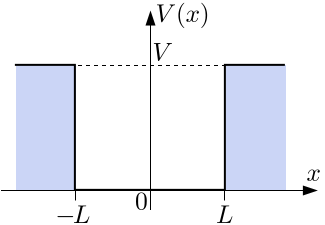
\includegraphics[width=0.4\textwidth]{Figures/03.png}
	\caption{}
	\label{fig:}
\end{figure}

denoted as Region I, II, and III with \(L = \frac{a}{2}\). Then we must have the following:

Region 1:
\[
	Ae^{ik_1 x} + Be^{-ik_1 x} 
\] 

Region 3:
\[
	E e^{ik_1 x} 
\]

Region 2:
\[
	C \sin k_2 x + D \cos  k_2 x
\]
We can now solve the boundary conditions where
\[
	k_1 = \sqrt{2m\frac{E-V_0}{\hbar ^{2} }} , k_2 = \sqrt{\frac{2mE}{\hbar ^{2} }} 
\]
\[
	\frac{\mathrm{d}\psi _1 }{\mathrm{d}x} (x= -\frac{a}{2}) = \frac{\mathrm{d}\psi _2}{\mathrm{d}x} (x= -\frac{a}{2})
\]
\[
	\psi _1 (x=-\frac{a}{2}) = \psi _2 (x=-\frac{a}{2})
\]
\[
	\frac{\mathrm{d}\psi _2}{\mathrm{d}x} \left( x =\frac{a}{2} \right)  = \frac{\mathrm{d}\psi _3}{\mathrm{d}x} \left( x = \frac{a}{2} \right)  
\]
\[
	\psi _2 \left( x=\frac{a}{2} \right) = \psi _3 \left( x= \frac{a}{2} \right) 
\]
Plugging in we have 
\[
	A e^{-ik_1 \frac{a}{2}} + Be^{ik_1 \frac{a}{2}} = -C \sin k_2 \frac{a}{2} + D \cos  k_2 \frac{a}{2}
\]
\[
	ik_1 \left[  Ae^{-ik_1 \frac{a}{2}} - Be^{ik_1 \frac{a}{2}}   \right] = k_2 \left[  C \cos  k_2 \frac{a}{2} + D \sin  k_2 \frac{a}{2} \right] 
\]
and the same with the other teams. Solving the algebra we will get the following: 
\[
	E = e^{-2i k_1 \frac{a}{2}} \cdot \frac{A}{\cos  k_2 a - i \frac{k_1 ^{2}  + k_2 ^{2}  }{2k_1 k_2} \sin  k_2 a} 
\]
\[
	\mathcal{T} = \vert \frac{E}{A} \vert ^{2} 
\]
which gives an oscillating probability

Plotting the transmission as a function of energy will give	
\begin{figure}[H]
	\centering
	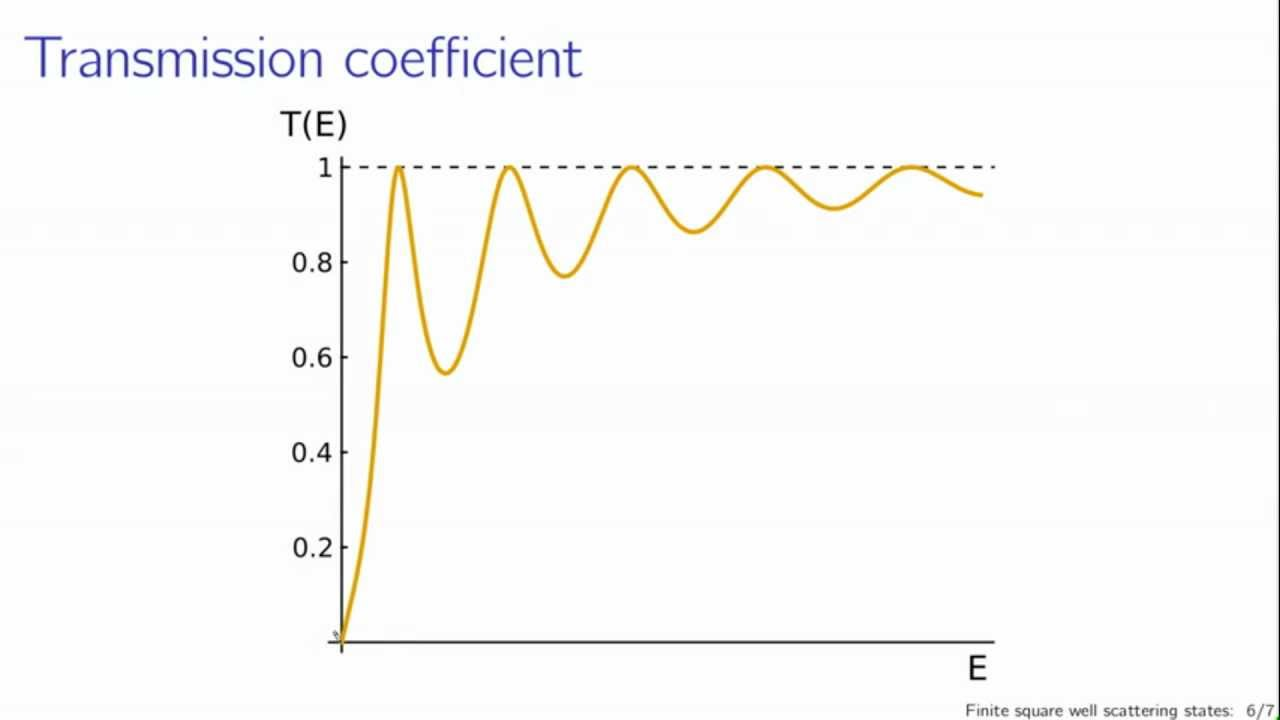
\includegraphics[width=0.5\textwidth]{Figures/06.jpg}
	\caption{}
	\label{fig:}
\end{figure}
We see we get a resonance where the particle can go through the potential. where the resonance will be where
\[
	k_2 = n \frac{\pi}{a}
\] 
This is such that the transmitting and reflecting wave match up to get a resonance. 
\begin{eg}
	Notice with semiconductors we can do this quite easily. When we inject an electron we can get a resonance tunneling where there is no resistance except the metal. Thus, the semiconductor doesn't exist. 
\end{eg}